\begin{frame}{Event pre-selection}
    \begin{columns}[onlytextwidth, t]
        \begin{column}{0.45\textwidth}
            \begin{align*}
                \mathtt{intensity} &> 300\\
                \mathtt{leakage1\_intensity} &< 0.2\\
                \mathtt{leakage2\_intensity} &< 0.2
            \end{align*}
            \begin{itemize}
                \item[\textbf{\textcolor{green}{+}}] Remove incomplete shower images
                \item[\textbf{\textcolor{green}{+}}] Remove dim events
                \item[\textbf{\textcolor{red}{-}}] Remove low energy events
            \end{itemize}
        \end{column}
        \begin{column}{0.45\textwidth}
            \only<2>{
                \begin{align*}
                    \mathtt{intensity} &> 150\\
                    \mathtt{leakage1\_intensity} &< 0.2\\
                    \mathtt{leakage2\_intensity} &< 0.2
                \end{align*}
                \begin{itemize}
                    \item[\textbf{\textcolor{green}{+}}] Lower energy events included
                    \item[\textbf{\textcolor{red}{-}}] which are harder to reconstruct
                \end{itemize}
            }
        \end{column}
    \end{columns}

    \note<1->[item]{Zuerst Eventselektion $\to$ diese Kriterien}
    \note<1->[item]{\texttt{leakage} $\to$ entferne unvollständige Bilder}
    \note<1->[item]{\texttt{intensity} $\to$ entferne dunkle Bilder (hell besser rekonstruierbar)}
    \note<2->[item]{Derart großer Wert für \texttt{intensity} $\to$ entfernt niederenergetische Ereignisse
        \newline $\to$ Wert verringern \newline
    }
    \note<2->[item]{Plots im Folgenden: v0.5.2 + \texttt{intensity > 300}}
\end{frame}

\begin{frame}{The aict-tools}
    \begin{columns}[onlytextwidth]
        \begin{column}{0.65\textwidth}
            \begin{itemize}
                \item Apply event pre-selection
                \item Train and apply scikit-learn models for 
                    \begin{itemize}
                        \item Gamma-hadron separation
                        \item Energy estimation
                        \item Origin reconstruction
                    \end{itemize}
                \item Create performance plots
            \end{itemize}
            \medskip
            \onslide<2->{
                Commandline applications \& configuration using a single YAML-file
                \begin{itemize}
                    \item[\textbf{\textcolor{tugreen}{\to}}] automated pipeline using make \textbf{\textcolor{tugreen}{\to}} reproducibility
                \end{itemize}
                Initially developed for FACT 
                \begin{itemize}
                    \item Different conventions than CTA (e.g. camera frame definition, units)
                        \begin{itemize}
                            \item[\textbf{\textcolor{tugreen}{\to}}] Conversion of LST data necessary
                        \end{itemize}
                    \item Continued development adds more CTA support 
                        \begin{itemize}
                            \item[\textbf{\textcolor{tugreen}{\to}}] Only data-structure adjustment and some renaming necessary now
                        \end{itemize}
                \end{itemize}
            }
        \end{column}
        \begin{column}{0.33\textwidth}
            \centering
            
\includegraphics[width=\textwidth]{images/python.png}
            
\includegraphics[width=0.8\textwidth]{images/scikit.png}
            
\includegraphics[width=\textwidth]{images/pandas.png}
        \end{column}
    \end{columns}
    \onslide<2->{
        \begin{center}
            \vspace{0.5\baselineskip}
            \small\fullcite{aict-tools}
        \end{center}
    }

    \note<1->[item]{Durchführung der Analyse: aict-tools}
    \note<1->[item]{- Eventselektion anwenden
        \newline - Modelle des ML trainieren \& anwenden 
        \newline - scikit-learn Modelle 
        \newline - für Teilchentypbestimmung, Energieschätzung und Richtungsrekonstruktion
        \newline - Performance plots
    }
    \note<2->[item]{Vorteil: Anwendung mit Kommandozeile \& Konfiguration mit 1 YAML-Datei
        \newline $\to$ Analyse automatisieren 
        \newline $\to$ Reproduzierbarkeit 
        \newline $\to$ + Hier: Vergleich Kombinationen
    }
    \note<2->[item]{Ursprünglich für FACT entwickelt 
        \newline $\to$ Andere Konventionen 
        \newline $\to$ LST Daten anpassen
        \newline $\to$ Während Arbeit: Weiterentwicklung 
        \newline $\to$ nur noch minimale Anpassungen nötig
    }
\end{frame}

\begin{frame}{The disp method}
    \begin{columns}[onlytextwidth]
        \begin{column}{0.475\textwidth}
            \begin{itemize}
                \setlength\itemsep{1em}
                \item Origin reconstruction is 2D regression task 
                \item Assuming the main shower axis is correctly reconstructed\\
                    \begin{itemize}
                        \item[\textbf{\textcolor{tugreen}{\to}}] Estimate distance along axis $\to$ 1D regession
                        \item[\textbf{\textcolor{tugreen}{\to}}] Decide which side of cog $\to$ classification
                    \end{itemize}
            \end{itemize}
        \end{column}
        \begin{column}{0.475\textwidth}
            \centering
            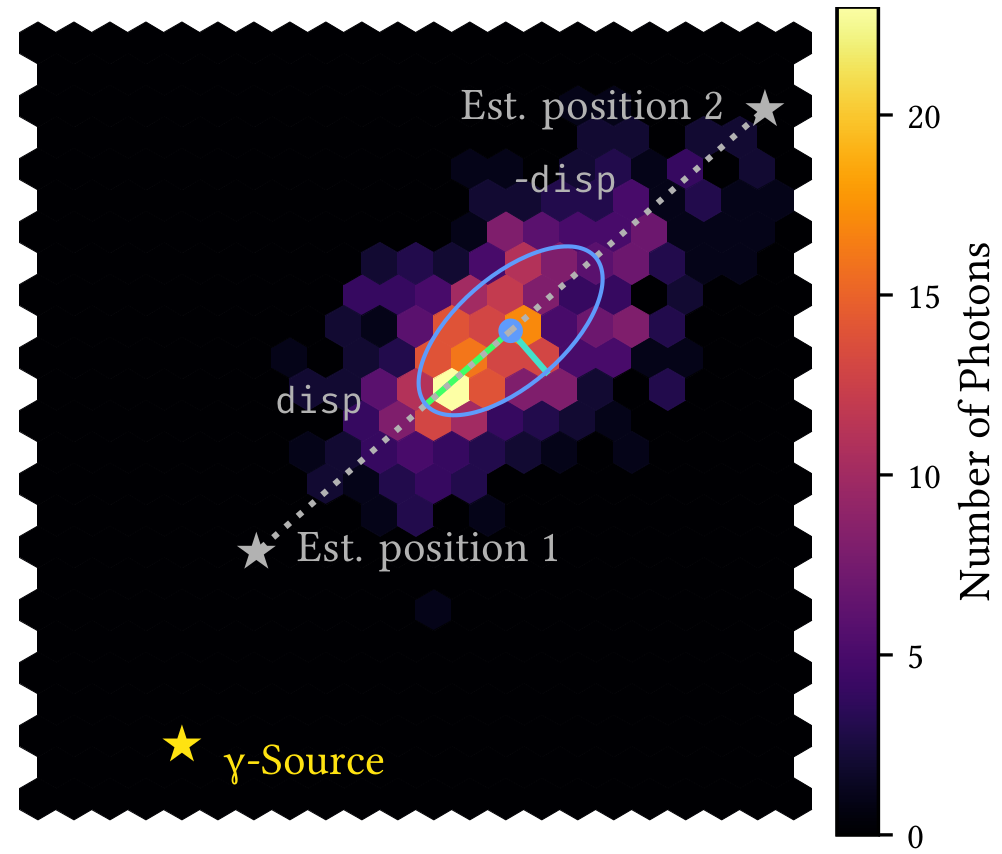
\includegraphics[width=\textwidth]{images/disp.png}\\[-0.5\baselineskip]
            \hspace{1.5cm}\href{https://github.com/MaxNoe/phd_thesis}{[Max Noethe, PhD thesis]}
        \end{column}
    \end{columns}

    \note[item]{Richtungsrekonstruktion aict-tools $\to$ disp Methode}
    \note[item]{Normalerweise 2D Regression}
    \note[item]{Annahme: Hauptachse korrekt rekonstruiert
        \newline $\to$ Abstand Quelle entlang Hauptachse
        \newline $\to$ + Entscheidung welche Seite von Schwerpunkt
    }
\end{frame}